\section{BUSCO Results}
\label{section:busco}

Results of BUSCO analysis using the sordariomycetes\_Odb12 dataset provided by BUSCO are presented in Figure~\ref{fig:busco-complete}, Figure~\ref{fig:busco-missing}, and Table~\ref{table:busco}. The results 
indicate that all gene sets considered in this analysis have a BUSCO
completeness of 94.9\% or higher, with a maximum completeness of
99.9\% in the case of Braker2 and DC1. In general, Braker2 and RefSeq have the
most BUSCO complete sets of gene predictions of the three tools
considered. Interestingly, Braker2 produces far more duplicated BUSCO
matches than both GeneMark and RefSeq. Examining the BUSCO output
logs, this appears to be due to Braker2 predicting more than one
coding sequence for some genes predictions, resulting in multiple
similar proteins. Interestingly, the coding sequences in the RefSeq annotations seem to miss far more genes than the other two gene finders while also having a higher number of fragmented BUSCO genes. This may be due to human curation of the RefSeq datasets, or the Gnomon gene prediction pipeline used by NCBI to produce these annotations. Further investigation is required to determine the exact cause of this discrepancy. Finally, it appears that \textit{T. reesei} tends to have slightly lower BUSCO completeness than the other \textit{Trichoderma} species considered in this analysis, regardless of gene finder used. Why this is the case is unknown, but may be due to the evolutionary distance between \textit{T. reesei}, the Gnomon annotation process, or potentially the fragmented nature of the \textit{T. reesei} assembly used in this analysis. 

In general, all gene finders perform
well in regards to BUSCO performance. While these results do not
capture the entire set of genes possibly present in these
\textit{Trichoderma} assemblies, they do confirm that the gene finders
are at minimum predicting many evolutionarily conserved fungal genes.

\begin{figure}
  \centering
  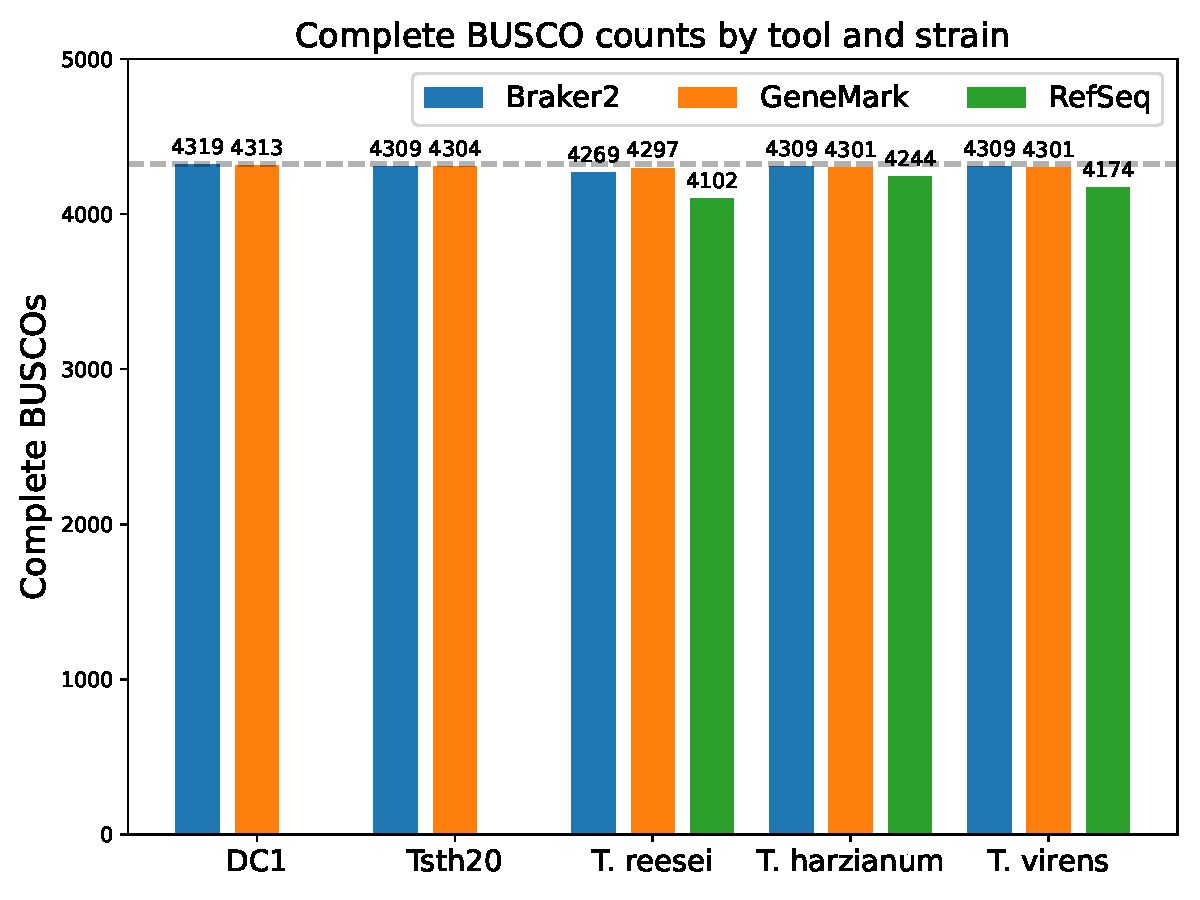
\includegraphics[width=0.90\textwidth]{figures/busco-complete-counts.pdf}
  \caption[Complete BUSCO counts]{Barplot showing the number of complete BUSCOs for each gene finder across all \textit{Trichoderma} genome assemblies. For DC1 and Tsth20, RefSeq annotations are not available, so their values are set to 0. The dashed line indicates the total number of BUSCO markers in the selected dataset (4323).}
  \label{fig:busco-complete}
\end{figure}

\begin{figure}
  \centering
  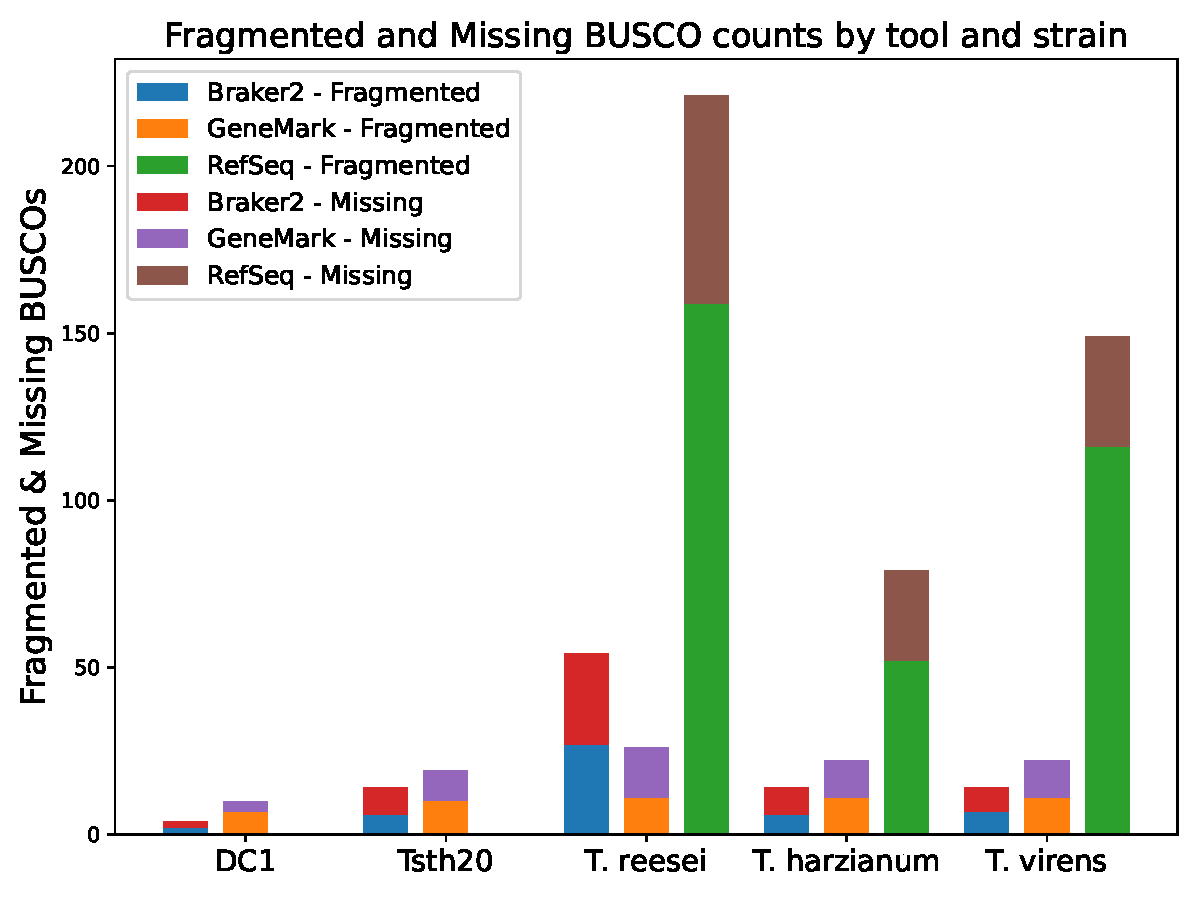
\includegraphics[width=0.90\textwidth]{figures/busco-missing-counts.pdf}
  \caption[Missing BUSCO counts]{Barplot showing the number of missing BUSCOs for each gene finder across all \textit{Trichoderma} genome assemblies. For DC1 and Tsth20, RefSeq annotations are not available, so their values are set to 0. The dashed line indicates the total number of BUSCO markers in the selected dataset (4323).}
  \label{fig:busco-missing}
\end{figure}

\begin{table}
  \begin{center}
    \begin{subtable}{\textwidth}
      \centering
      \begin{tabular}{|c|c|c|c|c|c|c|}
        \hline
        Strain & Complete & Single & Duplicated & Fragmented & Missing \\ \hline
        DC1 & 4319 & 3505 & 814 & 2 & 2 \\ \hline
        Tsth20 & 4309 & 3575 & 734 & 6 & 8 \\ \hline
        \textit{T. reesei} & 4269 & 3616 & 653 & 27 & 27 \\ \hline
        \textit{T. harzianum} & 4309 & 3562 & 747 & 6 & 8 \\ \hline
        \textit{T. virens} & 4309 & 3504 & 805 & 7 & 7 \\ \hline
      \end{tabular}
      \caption{Braker2}
      \vspace{0.5cm}
    \end{subtable}
    \begin{subtable}{\textwidth}
      \centering
      \begin{tabular}{|c|c|c|c|c|c|c|}
        \hline
        Strain & Complete & Single & Duplicated & Fragmented & Missing \\ \hline
        DC1 & 4313 & 4311 & 2 & 7 & 3 \\ \hline
        Tsth20 & 4304 & 4291 & 13 & 10 & 9 \\ \hline
        \textit{T. reesei} & 4297 & 4297 & 0 & 11 & 15 \\ \hline
        \textit{T. harzianum} & 4301 & 4291 & 10 & 11 & 11 \\ \hline
        \textit{T. virens} & 4301 & 4291 & 10 & 11 & 11 \\ \hline
      \end{tabular}
      \caption{GeneMark}
      \vspace{0.5cm}
    \end{subtable}
    \begin{subtable}{\textwidth}
      \centering
      \begin{tabular}{|c|c|c|c|c|c|c|}
        \hline
        Strain & Complete & Single & Duplicated & Fragmented & Missing \\ \hline
        \textit{T. reesei} & 4102 & 4101 & 1 & 159 & 62 \\ \hline
        \textit{T. harzianum} & 4244 & 4234 & 10 & 52 & 27 \\ \hline
        \textit{T. virens} & 4174 & 4164 & 10 & 116 & 33 \\ \hline  
      \end{tabular}
      \caption{RefSeq}
    \end{subtable}
  \end{center}
  \caption{Results from BUSCO using the fungal analysis option
    organized by gene finding tool. The selected BUSCO dataset
    contains 4323 markers. For more information on the categories
    assigned by BUSCO, please refer to the documentation.}
  \label{table:busco}
\end{table}

While BUSCO matches are a good metric for general performance of gene
finders, it is also important to investigate BUSCO proteins without
matching gene predictions. Table \ref{table:busco}, shows breakdowns
of genes missed by each gene finder across the \textit{Trichoderma}
assemblies. 


%\begin{center}
% \begin{table}
% \makebox[\textwidth]{
% \begin{tabular}{|c|c|c|c|c|c|c|c|}
%   \hline
%   Tool & BUSCO ID & Annotation & DC1 & Tsth20 & \textit{T. reesei} & \textit{T. harzianum} & \textit{T. virens} \\ \hline
%   Braker2 & 195619at4751 & \makecell{Pyridoxal phosphate-dependent \\ transferase} & \  & \checkmark & \checkmark & \checkmark & \checkmark \\ \hline
%   Braker2 & 285254at4751 & Aminoacyl-tRNA synthetase & \checkmark & \checkmark & \checkmark &  & \checkmark \\ \hline
%   Braker2 & 348020at4751 & Formyl transferase &  &  & \checkmark &  & \checkmark \\ \hline
%   Braker2 & 497024at4751 & Zinc finger C2H2-type &  & \checkmark & \checkmark & \checkmark & \checkmark \\ \hline
%   GeneMark & 195619at4751 & \makecell{Pyridoxal phosphate-dependent \\ transferase} &  & \checkmark & \checkmark & \checkmark & \checkmark \\ \hline
%   GeneMark & 285254at4751 & Aminoacyl-tRNA synthetase & \checkmark & \checkmark & \checkmark &  & \checkmark \\ \hline
%   GeneMark & 348020at4751 & Formyl transferase &  &  &  &  & \checkmark \\ \hline 
%   GeneMark & 438731at4751 & LSM domain & \checkmark & \checkmark &  & \checkmark & \checkmark  \\ \hline
%   GeneMark & 470813at4751 & Ubiquitin-conjugating enzyme &  &  &  &  &  \\ \hline
%   GeneMark & 497024at4751 & Zinc finger C2H2-type &  & \checkmark & \checkmark & \checkmark & \checkmark \\ \hline
%   RefSeq & 494at4751 & Midasin & N/A & N/A &  &  & \checkmark\\ \hline
%   RefSeq & 315802at4751 & tRNA dimethylallyltransferase & N/A & N/A & \checkmark & \checkmark &  \\ \hline
%   RefSeq & 352224at4751 & YEATS & N/A & N/A &  & \checkmark &  \\ \hline
% \end{tabular}
% }
% \caption[GeneMark missed BUSCO proteins]{The presence (\checkmark)
%   or absence of all BUSCO IDs missed by Braker2, GeneMark and RefSeq
%   in each \textit{Trichoderma} assembly.}
% \label{table:genemark-busco}
%\end{table}
%\end{center}

%\begin{table}
%  \centering
%  \begin{tabular}{|c|c|c|c|c|c|c|}
%    \hline
%    BUSCO ID & Annotation & DC1 & Tsth20 & \textit{T. reesei} & \textit{T. harzianum} & \textit{T. reesei} \\ \hline
%    494at4751 & Midasin & N/A & N/A & X & X & \checkmark\\ \hline
%    315802at4751 & tRNA dimethylallyltransferase & N/A & N/A & \checkmark & \checkmark & X \\ \hline
%    352224at4751 & YEATS & N/A & N/A & X & \checkmark & X \\ \hline
%  \end{tabular}
%  \caption[RefSeq missed BUSCO proteins]{The presence (\checkmark) or
%    absence (X) of all BUSCO IDs missed by RefSeq in each
%    \textit{Trichoderma} assembly.}
%  \label{table:refseq-busco}
%\end{table}

Braker2, GeneMark and RefSeq all demonstrate excellent coverage of the
BUSCO fungal protein set, indicating that these gene finders are
capable of predicting genes that are expected to be present in these
assemblies. From this we can say that the foundations of the
underlying gene models used by each gene finder are solid. Braker2
produces more duplicate matches than GeneMark and RefSeq, but this is
likely due to multiple isoforms of possible genes being present in the
input data. Despite excellent coverage of the BUSCO fungal proteins,
all three gene finders miss some BUSCO proteins in their
predictions. 
Finally, we reiterate the possibility that human curation of RefSeq datasets is responsible for these differences, but this requires further investigation.
